\begin{figure*}
    \vspace{-2mm}
    \centering
    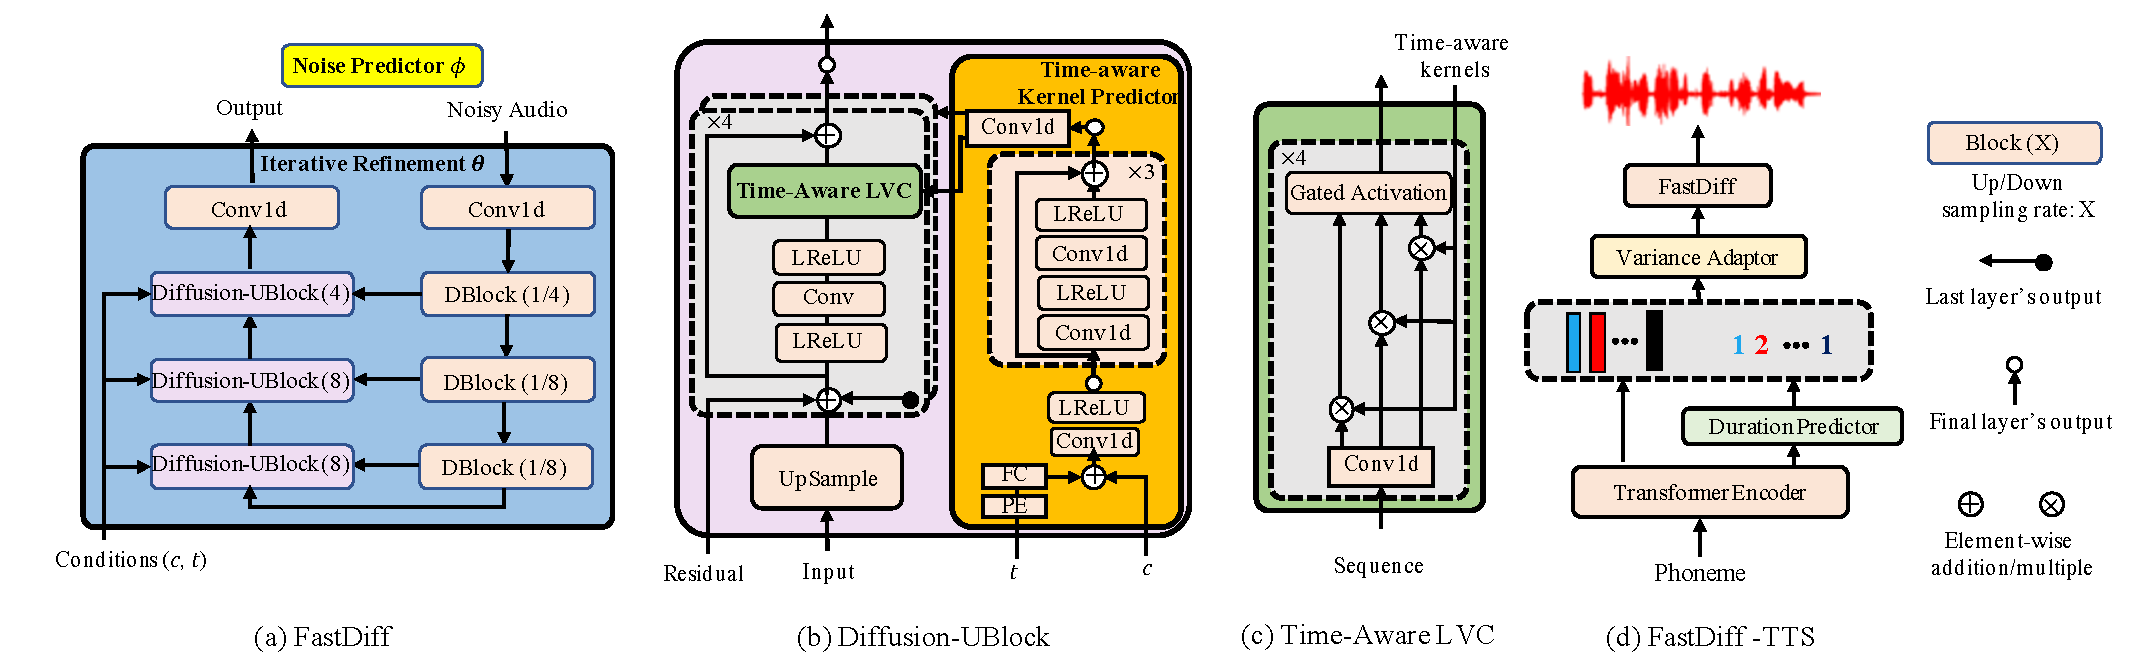
\includegraphics[width=0.95\textwidth,trim={1.0cm 0cm 1.0cm 0cm}]{Figures/arch1.pdf}
    \vspace{-1mm}
   \caption{The overall architecture for FastDiff and FastDiff-TTS. The refinement model $\theta$ in FastDiff takes noisy audio $\vx_{t}$ as input and computes $\beps_{\theta}(\vx_{t}|c, t)$ conditioned on diffusion time index $t$ and Mel-spectrogram $c$. We use LReLU to denote the leaky rectified linear unit, LVC to denote the location-variable convolution, FC to denote the fully-connected layer, and PE to denote the positional encoding operation.} 
%   \vspace{-2mm}
    \label{fig:arch}
  \end{figure*}


\section{FastDiff}
This section presents our proposed FastDiff, a fast conditional diffusion model for high-quality speech synthesis. We first describe the motivation of the design in FastDiff. Secondly, we introduce the iterative refinement model $\theta$ for high-quality speech synthesis and the noise predictor $\phi$ for accelerated sampling. Furthermore, we describe the training and inference procedures in detail. At last, we extend FastDiff to FastDiff-TTS for fully end-to-end text-to-speech syntheses.

\subsection{Motivation}
While denoising diffusion probabilistic models have shown high potential in synthesizing high-quality speech samples \cite{chen2020wavegrad,kong2020diffwave,liu2021diffsinger}, several challenges remain for industrial deployment: 1) Different from the traditional generative models, diffusion models catch dynamic dependencies from noisy audio instead of clean ones, which introduce more variation information (i.e, noise levels) in addition to the spectrogram fluctuation. 2) With limited receptive field patterns, a distinct degradation could emerge when reducing the reverse iterations, making diffusion models difficult to get accelerated. As a result, hundred or thousand orders of iterations prevent existing diffusion models from real-world deployment.

In FastDiff, we propose two key components to complement the above issues: 1) FastDiff adopts a time-aware location-variable convolution to catch the details of noisy samples at dynamic dependencies. The convolution operations are conditioned on dynamic variations in speech including diffusion steps and spectrogram fluctuations, equipping the model with diverse receptive field patterns and promoting the robustness of diffusion models during reverse acceleration. 2) To accelerate the inference procedure, FastDiff adopts a noise schedule predictor to reduce the number of reverse iterations, frees diffusion models from hundreds or thousands of refinement iterations. This makes FastDiff for the first time applicable to interactive, real-world applications at a low computational cost.

% further adopt a noise schedule predictor to reduce the number of reverse iteration and computational costs. 
% FastDiff mainly consists of several techniques to achieve high quality, fast and diverse speech synthesis, including diffusion dynamic convolution and accelerated sampling. 1) To improve audio quality, FastDiff adopts diffusion dynamic convolution to catch the details of noisy samples at dynamic dependencies. The convolution operations are conditioned on dynamic variations in speech including diffusion steps and spectrogram fluctuations, equipping model with diverse receptive field patterns and premoting the robustness of diffusion models during reverse acceleration. 

\subsection{Time-Aware Location-Variable Convolution}

% To efficiently capture time dependent features, diverse receptive field patterns are essential for high-fidelity wavefrom synthesis, which should be extensive to catch long dependencies in audio. Location-variable convolution is efficient in capturing the long dependencies of audio through convolutions on multiple intervals, resulting in enhanced sound quality as well as speed. 

In comparison with traditional convolution networks, location-variable convolution~\cite{zeng2021lvcnet} shows efficiency in modeling the long-term dependency of audio and gets neural network free from a significant number of dilated convolution layers. Inspired by this, we introduce the Time-Aware Location-Variable Convolution, which is sensitive to time steps in diffusion probabilistic models. At time step $t$, we follow~\cite{vaswani2017attention} to embed the step index into an 128-dimensional positional encoding (PE) vector $\ve_t$:
\begin{align*}
\ve_t=&\left[\sin \left(10^{\frac{0 \times 4}{63}} t\right), \cdots, \sin \left(10^{\frac{63 \times 4}{63}} t\right),\right.\\
&\,\,\left.\cos \left(10^{\frac{0 \times 4}{63}} t\right), \cdots, \cos \left(10^{\frac{63 \times 4}{63}} t\right)\right],
\end{align*}

In time-aware location-variable convolution, FastDiff requires multiple predicted variation-sensitive kernels to perform convolutional operations on the associated intervals of input sequence. These kernels should be time-aware and sensitive to variations of noisy audio including diffusion steps and acoustic features (i.e., Mel-spectrogram). Therefore, we propose a time-aware location-variable convolution (LVC) module, which is coupled with a kernel predictor as shown in Figure~\ref{fig:arch}(b) and Figure~\ref{fig:arch}(c). We describe the overall calculations below.

For the $q$-th time-aware LVC layer, we split the input $\vx_t\in\sR^{D}$ using a $M$-length window with $3^q$ dilations to produce $K$ segments with each $\vx_{t}^{k}\in\sR^M$:
  \begin{equation}
    \{\vx_{t}^{1}, \ldots, \vx_{t}^{K}\}=\operatorname{split}(\vx_t;M, q)
\end{equation}

Next, we perform convolutional operations on the associated intervals of input sequence using the kernels generated by a kernel predictor $\alpha$:
\begin{align}
    \{ \mF_{t}, \mG_{t}\} &= \alpha (t, c) \\ 
    \boldsymbol{z}_{t}^{k} &=\tanh (\boldsymbol{F}_{t} *  \boldsymbol{x}_{t}^{k}) \odot \sigma(\boldsymbol{G}_{t} *  \boldsymbol{x}_{t}^{k})\\
    \boldsymbol{z}_{t}&=\operatorname{concat}(\{\boldsymbol{z}_{t}^{1}, \ldots, \boldsymbol{z}_{t}^{K}\}),
\end{align}
where $\boldsymbol{F}_{t}, \boldsymbol{G}_{t}$ denote the filter and the gate kernels for $\vx_t^i$, respectively, $*$ denotes the 1d convolution, $\odot$ denotes the element-wise product and $\operatorname{concat}(\cdot)$ denotes the concatenation between vectors. Since the time-aware kernels are adaptive to the noise-level and dependent to the acoustic features, FastDiff is capable of precisely estimating de-noising gradient with a superior speed given a noisy signal input.

\subsection{Accelerated Sampling}

\subsubsection{Noise Predictor}
To avoid sampling with hundreds to thousands steps, FastDiff adopts the noise scheduling algorithm in the bilateral denoising diffusion models (BDDMs)~\cite{lam2022bddm} to predict a sampling noise schedule much shorter than the noise schedule used in training. This scheduling method has been revealed to be superior than other sampling acceleration methods, e.g.,  the grid search algorithm in WaveGrad~\cite{chen2020wavegrad} and the fast sampling algorithm in DiffWave~\cite{kong2020diffwave}. The noise predictor iteratively derives a continuous noise schedule $\hat{\mBeta}\in\sR^{T_m}$. We attach the learning objective and corresponding likelihood in Appendix~\ref{appendix:diffusion}. 

\subsubsection{Schedule Alignment} \label{schedule}

In FastDiff, similar to DDPMs, during training we use $T=1000$ discrete time steps. Therefore, when needed to condition on $t$ during sampling, we also need to approximate $T_m$ discrete time indices by aligning the $T_m$-step sampling noise schedule $\hat{\mBeta}$ to the $T$-step training noise schedule $\mBeta$, with $N<<T$. We have attached the detailed algorithms in Appendix~\ref{appendix:Training}. 

% before inference. To be more specific, given tighter and more efficient continuous noise schedule $\hat{\beta}$, it should generate 

    % \begin{algorithm}[h]
    %     \centering
    %     \caption{Training}\label{alg: training}
    %     \textbf{Input}: Pre-defined discrete $\beta$, iterative refinement model $\theta$, noise schedule predictor $\phi$ and refinement postnet $\alpha$. 
    %     \begin{algorithmic}[1]
    %     \REPEAT 
    %     \STATE Sample $x_{0} \sim q_{data}$, $\epsilon\sim\gN(0,I)$, and\\ \quad $t\sim\mathrm{Uniform}(\{1,\cdots,T\})$
    %     \STATE Take gradient descent steps on $\nabla_{\theta} \gL_{\theta}$ according to \eqref{eq: score_loss}.
    %     \IF{Training steps $>$ 20k} 
    %     \STATE Take gradient descent steps on $\nabla_{\phi} \gL_{\phi}$ according to \eqref{eq: noise_loss}.
    %     \ENDIF 
    %     \UNTIL{iterative refinement model $\theta$, noise schedule predictor $\phi$ converged}
    %     \vspace{0.09em}
    %     \end{algorithmic}
    %     \end{algorithm}


\subsection{Training, Noise Scheduling and Sampling}

All illustrated in Algorithm~\ref{alg: training}, we separately parameterize FastDiff by two modules: 1) a iterative refinement model $\theta$ that minimizes a variational bound of the score function, and 2) a noise predictor $\phi$ that optimizes the noise schedule for a tighter evidence lower bound. For inference, we first derive the tighter and more efficient noise schedules $\hat{\beta}$ via an one-shot noise scheduling procedure, which makes FastDiff achieve orders of magnitude faster at sampling. It has been demonstrated~\cite{lam2022bddm} that the noise schedule searched for as few as 1 sample could be robust enough to maintain a high-quality generation among all samples in testing set. Secondly, we map the continuous noise schedules to discrete time indexes $T_m$ using schedule alignment. Finally, FastDiff iteratively refines gaussian noise to generate high-quality samples with computational efficiency. The detailed information on training, noise scheduling and inference procedures has been presented in Appendix~\ref{appendix:schedule_alignment}.

